\chapter{ClickNP编程平台介绍}
\section{系统架构}
ClickNP基于Catapult Shell体系结构搭建。该体系结构包含PCIe、直接内存访问(direct memory access, DMA)、
内存管理单元(memory management unit, MMU)、以太网介质访问控制(media access control, MAC)等
适用于多种应用场景的可服用逻辑,并将其抽象为定义好的接口。由ClickNP编写的FPGA程序生成的目标为Catapult功能。
由于ClickNP依赖的不同高级编程工具生成的目标接口不一致,因此在其下层有一个适配层,
将不同高级编程工具接口统一到Catapul Shell接口。

主机进程通过ClickNP库函数与FPGA程序通信,而库函数则依赖Catapult PCIe接口实现。
ClickNP库主要实现两个重要的功能:主机与FPGA之间的高速低延迟PCIe通道应用程序接口,
以及不同高级编程工具向FPGA模块传递参数并发送启动、停止、复位等信号的调用接口。

主机进程包括一个管理线程以及零个或多个工作线程。管理进程负责将程序镜像载入硬件、
启动工作进程、根据配置初始化FPGA和CPU中的ClickNP元件以及在运行时通过想各个元件发送信号来控制其行为。
在CPU的指派下,每个工作线程可以处理多个任务。

\section{程序设计}
\subsection{概念抽象}
ClickNP提供了模块化的编程模型,以元件为基本处理模块。每个元件包括以下属性:
\begin{description}
\item[本地状态]每个元件可定义一系列仅由自身访问的本地状态;
\item[输入输出端口]一个元件可以通过多个输入输出端口与其他元件通信;
\item[句柄函数]一个元件有三个句柄函数:初始化函数只在元件启动时执行一次;
处理函数在元件工作期间反复调用,处理输入的数据;信号函数类似于中断控制器,
在元件从主机进程收到信号时被调用,处理指令。
\end{description}

一个元件的输出端口可以用通道与另一个元件的输入端口连接。在ClickNP中,通道相当于一个先进先出的缓冲区,
从其一端写入,从另一端读取,如图~\ref{fig:channel}所示。
\begin{figure}[ht]
\centering
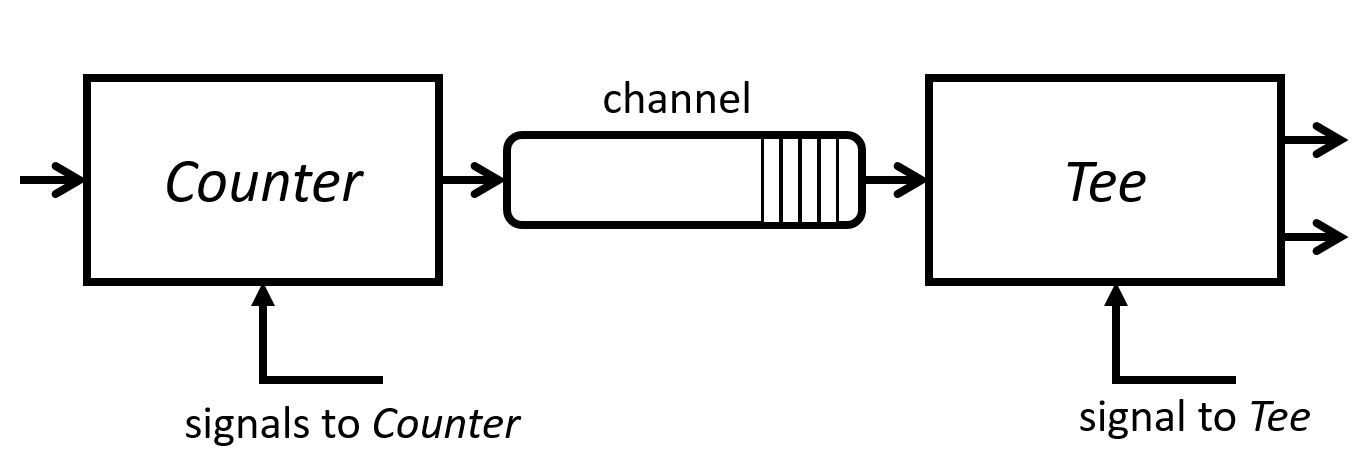
\includegraphics[width=4in]{channel}
\caption{连接两个元件的通道} \label{fig:channel}
\end{figure}

每次通道读写操作的基本单位为帧,每个帧的大小固定为64字节,其中头部包含元数据,
数据载荷长32字节。其结构及成员定义如图~\ref{fig:flit}、图~\ref{fig:flitdef}所示。
\begin{figure}[ht]
\centering
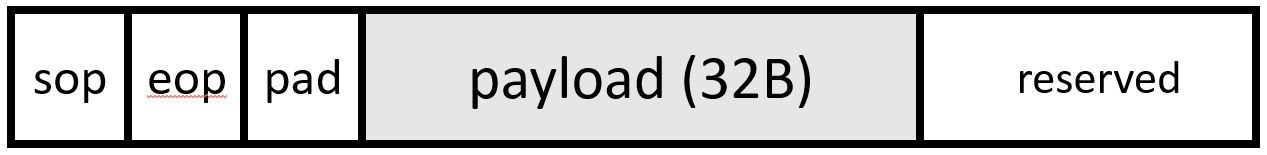
\includegraphics[width=4in]{flit}
\caption{帧结构} \label{fig:flit}
\end{figure}

\begin{figure}[ht]
\centering
\lstinputlisting{code/flit.cl}
\caption{帧成员定义} \label{fig:flitdef}
\end{figure}

以完整包为代表的大段数据会被拆分为多个帧在元件之间传播。
其中第一帧的包开始位(start of packet, \lstinline$sop$)置为真,
最后一帧的包结束位(end of packet, \lstinline$eop$)置为真。
如果数据载荷小于32字节,那么最后一帧的留白(padding, \lstinline$pad$)域指代载荷的尾部留白区段大小。
将大的包拆分为帧,不仅能够降低延迟,还有助于提升处理包数据的各级流水线之间并行化程度。

在定义完各个元件之后,通过ClickNP配置文件将元件连接为有向图,使其互连,形成总的计算系统,
图~\ref{fig:cfg}为一个远程直接内存访问(remote direct memory access, RDMA)处理器的配置文件,
其开头部分描述该系统依赖的元件类型,随后将元件实例化,并用箭头表示其通道连接关系,
自左侧元件的输出端口指向右侧元件的输入端口,方括号中的数字代表端口号。
\begin{figure}[ht]
\centering
\lstinputlisting{code/RoCE.cfg}
\caption{ClickNP配置文件示例} \label{fig:cfg}
\note{第8行\lstinline$host$关键字代表将\lstinline$RoCE_Connector$元件实例化为主机工作线程}
\end{figure}

\subsection{编程语言}
ClickNP元件类似于面向对象语言中的对象,可以用C++这样的语言定义。
但现有的很多高级编程工具只支持C语言,而将高级语言转化为C语言的工作是乏味的,
因此我们采用的是针对定义元件的需要对C语言进行扩展这种途径。

图~\ref{fig:count}是一个包计数器元件的定义。\lstinline$.element$关键字定义元件名称;
尖括号内为输入输出端口数;\lstinline$.state$关键字定义本地状态\lstinline$count$计数器;
\lstinline$.init$关键字定义初始化函数,将\lstinline$count$的初值置零;
\lstinline$.handler$关键字定义处理函数,每当收到帧的\lstinline$sop$域为真时将计数器加一;
\lstinline$.signal$关键字定义信号函数,每当收到主机发来的任意信号帧时,
将当前包计数作为信号载荷发给主机。

ClickNP内建了一系列与端口进行数据交互的函数接口,如表~\ref{tab:operations}所示。
\begin{table}[htbp]
\centering
\caption{ClickNP内建接口} \label{tab:operations}
\begin{tabular}{l|l}
\hline
\lstinline$uchar get_input_port()$         & 获取第一个有帧输入的端口号 \\
\hline
\lstinline$bool test_input_port(uchar id)$ & 检查\lstinline$id$号端口有无帧输入 \\
\hline
\lstinline$flit read_input_port(uchar id)$ & 自\lstinline$id$号端口读取帧 \\
\hline
\lstinline$flit peek_input_port(uchar id)$ & 窥视\lstinline$id$号输入端口的帧 \\
\hline
\lstinline$void set_output_port(uchar id,$ & 向\lstinline$id$号端口写入帧, \\
\lstinline$flit x)$                        & 在处理函数执行到返回时, \\
                                           & 该帧将被写入通道 \\
\hline
\lstinline$ClSignal read_signal()$         & 自信号输入端口读取帧 \\
\hline
\lstinline$void set_signal(ClSignal p)$    & 向信号输出端口写入帧 \\
\hline

\hline
\end{tabular}
\end{table}

\begin{figure}[ht]
\centering
\lstinputlisting{code/Count.cl}
\caption{包计数器元件定义} \label{fig:count}
\end{figure}

\subsection{编译工具链}
ClickNP工具链以ClickNP编译器为前端,以Visual Studio、GCC等C/C++编译器、
Altera OpenCL SDK、Xilinx Vidado HLS等高级编程工具为后端。
开发人员需要完成三部分工作:
\begin{enumerate}
\item 定义元件,每个元件实现一小部分简单的功能;
\item 编写配置文件,描述元件之间的连接关系,以组成完整的逻辑系统;
\item 设计主机管理进程,初始化各元件并在运行时根据用户输入控制元件行为。
\end{enumerate}

以上三部分源程序由ClickNP编译器翻译为主机程序和FPGA程序两部分中间代码。
前者可由普通的C/C++编译器编译为目标文件,
后者需要由商业化高级编程工具合成为FPGA目标文件。
